\documentclass[12pt, titlepage]{article}

\usepackage{amsmath, mathtools}

\usepackage{amsfonts}
\usepackage{amssymb}
\usepackage{graphicx}
\usepackage{gensymb}
\usepackage{colortbl}
\usepackage{xr}
\usepackage{hyperref}
\usepackage{longtable}
\usepackage{xfrac}
\usepackage{xfrac}
\usepackage{tabularx}
\usepackage{float}
\usepackage{siunitx}
\usepackage{booktabs}
\usepackage{multirow}
\usepackage[section]{placeins}
\usepackage{caption}
\usepackage{fullpage}
\usepackage{cite}
\usepackage{breqn}

\input{../../Comments}
\input{../../Common}

\externaldocument[SRS-]{../../SRS/SRS}

\begin{document}

\title{Software Report\\\progname}

\author{\authname}

\date{}

\maketitle

\pagenumbering{roman}

\newpage
\section{Revision History}

\begin{table}[hp]
\caption{Revision History} \label{TblRevisionHistory}
\begin{tabularx}{\textwidth}{llX}
\toprule
\textbf{Date} & \textbf{Developer(s)} & \textbf{Change}\\
\midrule
Mar 7, 2026 & Kalp & Direction of Arrival theory and prototyping sections.\\
\bottomrule
\end{tabularx}
\end{table}

\newpage

\tableofcontents

\listoftables

\listoffigures

\newpage

\pagenumbering{arabic}

\section{Introduction}
\wss{Explain the purpose of this document. Why it was selected for this project.}
\wss{Briefly outline the structure of the document.}

\section{Direction of Arrival} \label{sec:doa}

Direction of arrival (DoA) estimation is a fundamental capability of \progname{}.
Given synchronized multi-channel audio from a microphone array, the system must
estimate the angular direction of sound sources on a 2D horizontal plane
relative to the user (\hyperref[SRS-FR5_2]{FR5.2}, \hyperref[SRS-FR5_3]{FR5.3}).
This section presents the theoretical foundations of the DoA algorithms used in
the project and describes the Python prototyping workflow employed to validate
and compare them.

\subsection{DoA Theory} \label{sec:doa_theory}

The DoA problem can be stated as follows. Let $\mathbf{x}_m(t)$ denote the
signal received at microphone $m$ at time $t$, for $m = 1, \ldots, M$ and $M
\geq 2$. A sound source at position $\mathbf{p}_s$ emits a signal $s(t)$ that
propagates through the medium. Due to the finite speed of sound $c$, the signal
arrives at each microphone with a time delay $\tau_m = \|\mathbf{p}_m -
\mathbf{p}_s\| / c$, where $\mathbf{p}_m$ is the position of microphone $m$.
The received signal is a delayed, attenuated, and possibly reverberant version
of the source. Estimating the direction of arrival amounts to inferring the
direction vector from the array center toward the source from the observed
multi-channel signals.

The project employs four DoA algorithms: Generalized Cross-Correlation with
Phase Transform (GCC-PHAT), Multiple Signal Classification (MUSIC), Steered
Response Power with Phase Transform (SRP-PHAT), and FRI-based DOA (FRIDA). Each
algorithm is described below.

\subsubsection{GCC-PHAT (Generalized Cross-Correlation with Phase Transform)}
\label{sec:gccphat}

GCC-PHAT estimates the time difference of arrival (TDOA) between pairs of
microphones. For a single source in the far field, the TDOA between microphones
$i$ and $j$ is related to the source direction by the geometry of the array.
Given TDOAs for multiple pairs, the source direction can be recovered via
triangulation or closed-form solutions for specific array layouts
\cite{Knapp1976GCC}.

Let $x_i(n)$ and $x_j(n)$ denote the discrete-time signals from microphones
$i$ and $j$, with sampling frequency $f_s$. The cross-correlation between them
is
\begin{equation}
  R_{ij}(\tau) = \mathbb{E}\left[ x_i(n) \, x_j(n + \tau) \right].
\end{equation}
In the frequency domain, the cross-power spectral density is
\begin{equation}
  G_{ij}(f) = X_i(f) \, \overline{X_j(f)},
\end{equation}
where $X_i(f)$ and $X_j(f)$ are the Fourier transforms of $x_i$ and $x_j$, and
$\overline{\cdot}$ denotes complex conjugation. The generalized
cross-correlation (GCC) with a weighting function $\Psi(f)$ is
\begin{equation}
  R_{ij}^{(\Psi)}(\tau) = \int_{-\infty}^{\infty} \Psi(f) \, G_{ij}(f) \,
  e^{j 2\pi f \tau} \, df.
\end{equation}

The Phase Transform (PHAT) weighting discards magnitude and retains only phase
information:
\begin{equation}
  \Psi_{\mathrm{PHAT}}(f) = \frac{1}{\left| G_{ij}(f) \right| + \epsilon},
\end{equation}
where $\epsilon > 0$ is a small constant to avoid division by zero. This
yields
\begin{equation}
  R_{ij}^{\mathrm{PHAT}}(\tau) = \int_{-\infty}^{\infty}
  \frac{G_{ij}(f)}{\left| G_{ij}(f) \right| + \epsilon} \,
  e^{j 2\pi f \tau} \, df.
\end{equation}
The TDOA estimate is the lag that maximizes the GCC-PHAT:
\begin{equation}
  \hat{\tau}_{ij} = \frac{1}{f_s} \cdot \arg\max_{\ell \in [-\ell_{\max},
  \ell_{\max}]} R_{ij}^{\mathrm{PHAT}}(\ell),
\end{equation}
where $\ell_{\max} = \lceil \tau_{\max} f_s \rceil$ and $\tau_{\max}$ is the
maximum physically feasible delay given the inter-microphone distance. In
practice, the integral is computed via the inverse FFT of the weighted
cross-spectrum.

For a rectangular four-microphone array, pairs $(1,2)$ and $(4,3)$ provide
horizontal-axis TDOAs; pairs $(3,2)$ and $(4,1)$ provide vertical-axis TDOAs.
The normalized delays $d_x$ and $d_y$ are averaged over each axis and converted
to an azimuth angle $\theta$ via $\theta = \arctan2(d_y, d_x) - \pi/2$, with
appropriate coordinate alignment for the glasses frame.

\subsubsection{MUSIC (Multiple Signal Classification)} \label{sec:music}

MUSIC is a subspace-based, high-resolution DoA algorithm \cite{Schmidt1986}. It
exploits the structure of the spatial covariance matrix to separate signal and
noise subspaces.

The received signal vector at frequency $f$ is modeled as
\begin{equation}
  \mathbf{x}(f) = \mathbf{A}(\theta) \, \mathbf{s}(f) + \mathbf{n}(f),
\end{equation}
where $\mathbf{A}(\theta) = [\mathbf{a}(\theta_1), \ldots, \mathbf{a}(\theta_D)]$
is the $M \times D$ steering matrix for $D$ sources, $\mathbf{a}(\theta)$ is
the steering vector for direction $\theta$, $\mathbf{s}(f)$ is the $D \times 1$
source vector, and $\mathbf{n}(f)$ is additive noise. For a plane wave from
direction $\theta$, the steering vector has elements
\begin{equation}
  a_m(\theta) = \exp\left( j \, \frac{2\pi f}{c} \, \mathbf{r}_m^\top
  \mathbf{u}(\theta) \right),
\end{equation}
where $\mathbf{r}_m$ is the position of microphone $m$ and $\mathbf{u}(\theta)$
is the unit direction vector.

The spatial covariance matrix is
\begin{equation}
  \mathbf{R}_x = \mathbb{E}\left[ \mathbf{x} \mathbf{x}^H \right] =
  \mathbf{A} \mathbf{R}_s \mathbf{A}^H + \sigma_n^2 \mathbf{I},
\end{equation}
where $\mathbf{R}_s$ is the source covariance matrix and $\sigma_n^2$ is the
noise power. Eigenvalue decomposition yields
\begin{equation}
  \mathbf{R}_x = \mathbf{U}_s \boldsymbol{\Lambda}_s \mathbf{U}_s^H +
  \mathbf{U}_n \boldsymbol{\Lambda}_n \mathbf{U}_n^H.
\end{equation}
The columns of $\mathbf{U}_s$ span the signal subspace (corresponding to the
$D$ largest eigenvalues); the columns of $\mathbf{U}_n$ span the noise
subspace. The key property is that steering vectors for true source directions
are orthogonal to the noise subspace: $\mathbf{a}^H(\theta) \mathbf{U}_n
\mathbf{U}_n^H \mathbf{a}(\theta) = 0$ when $\theta$ is a true DoA.

The MUSIC spatial spectrum is
\begin{equation}
  P_{\mathrm{MUSIC}}(\theta) = \frac{1}{\mathbf{a}^H(\theta) \,
  \mathbf{U}_n \mathbf{U}_n^H \, \mathbf{a}(\theta)}.
\end{equation}
DoA estimates are the $D$ peaks of $P_{\mathrm{MUSIC}}(\theta)$ over the search
range. MUSIC requires knowing or estimating $D$ and performs an eigendecomposition
per frequency bin; it offers high angular resolution but is sensitive to
model mismatch and coherent sources.

\subsubsection{SRP-PHAT (Steered Response Power with Phase Transform)}
\label{sec:srpphat}

SRP-PHAT is a beamforming-based method that searches over candidate source
positions to maximize the output of a steered delay-and-sum beamformer
\cite{DiBiase2000}. It is robust to reverberation and noise because the PHAT
weighting emphasizes phase coherence over magnitude.

For a candidate source position $\mathbf{x}$, the time difference of arrival
between microphones $m_1$ and $m_2$ is
\begin{equation}
  \tau_{m_1,m_2}(\mathbf{x}) = \frac{1}{c} \left( \|\mathbf{x} -
  \mathbf{p}_{m_1}\| - \|\mathbf{x} - \mathbf{p}_{m_2}\| \right).
\end{equation}
The steered response power at $\mathbf{x}$ is the sum of generalized
cross-correlations evaluated at the corresponding TDOAs:
\begin{equation}
  P(\mathbf{x}) = \sum_{m_1=1}^{M} \sum_{m_2=1}^{M} R_{m_1,m_2}^{\mathrm{PHAT}}
  \bigl( \tau_{m_1,m_2}(\mathbf{x}) \bigr).
\end{equation}
With PHAT weighting, each $R_{m_1,m_2}^{\mathrm{PHAT}}$ uses only phase
information, reducing sensitivity to spectral coloration and reverberation.

The source position estimate is
\begin{equation}
  \hat{\mathbf{x}}_s = \arg\max_{\mathbf{x} \in \mathcal{G}} P(\mathbf{x}),
\end{equation}
where $\mathcal{G}$ is a grid of candidate positions (e.g., on a sphere or
circle for 2D azimuth). The DoA is then the direction from the array center to
$\hat{\mathbf{x}}_s$. SRP-PHAT avoids eigendecomposition but requires a grid
search; resolution is limited by grid spacing and computational cost.

\subsubsection{FRIDA (FRI-Based DOA)} \label{sec:frida}

FRIDA leverages the finite rate of innovation (FRI) framework to estimate DoA
without a grid search \cite{Pan2017FRIDA}. It is designed for arbitrary
microphone array geometries and coherently combines multi-band information.

The central insight is that for any array layout, entries of the spatial
covariance matrix can be linearly transformed into a uniformly sampled sum of
sinusoids. The frequencies of these sinusoids encode the DoA. Specifically,
for a given frequency bin, the covariance between microphones $i$ and $j$
depends on the phase difference $\phi_{ij}(\theta) = (2\pi f / c) \,
(\mathbf{r}_i - \mathbf{r}_j)^\top \mathbf{u}(\theta)$. By arranging covariance
entries in a suitable structure, one obtains a signal of the form $\sum_d
\alpha_d e^{j \omega_d n}$, where $\omega_d$ is related to the $d$-th source
direction. FRI sampling theory allows recovery of $\omega_d$ from a small number
of samples, and thus recovery of the DoA, without exhaustive search.

FRIDA achieves state-of-the-art resolution at low signal-to-noise ratios by
coherently combining information across frequency bands. It supports both 2D
(azimuth only) and 3D (azimuth and elevation) localization and handles multiple
sources. The algorithm is implemented in the pyroomacoustics library
\cite{pyroomacoustics}.

\subsection{DoA Python Prototyping} \label{sec:doa_prototyping}

Before implementing DoA on the embedded microcontroller, the team developed a
Python prototyping pipeline to validate algorithms, compare their performance,
and generate labeled test data. This pipeline uses PyRoomAcoustics
\cite{pyroomacoustics} to simulate acoustic propagation in a 3D room and
produces multi-channel recordings that mimic what the microphone array would
capture in real conditions.

\subsubsection{Room Simulation with PyRoomAcoustics}

PyRoomAcoustics provides a \texttt{ShoeBox} room model: a rectangular enclosure
with configurable dimensions and acoustic properties. The simulation computes
room impulse responses (RIRs) between sources and microphones using the image
source method, which models reflections from walls, floor, and ceiling. The
received signal at each microphone is the convolution of the source signal with
the corresponding RIR, plus optional diffuse noise.

The prototyping code (in \texttt{src/prototyping/pyroomacoustics\_sim/}) creates
a room with dimensions $10 \times 10 \times 3$ metres and sampling frequency
$f_s = 8000$~Hz (or 16~kHz in the continuous simulation). Four microphones are
placed in a square configuration approximating the glasses form factor:
\begin{itemize}
  \item Microphone 1: $(4.95, 5.10, 1.75)$~m (front-left)
  \item Microphone 2: $(5.05, 5.10, 1.75)$~m (front-right)
  \item Microphone 3: $(4.95, 5.00, 1.75)$~m (back-left)
  \item Microphone 4: $(5.05, 5.00, 1.75)$~m (back-right)
\end{itemize}
The array spans approximately 10~cm in each horizontal dimension, consistent
with the physical spacing of microphones on the smart glasses.

A sound source is placed at a known position (e.g., $(9, 9, 1)$~m or
$(1, 6, 1)$~m). The source signal can be a sine wave, a pre-recorded audio file
(e.g., \texttt{car\_horn\_8k.mp3}), or live microphone input. The
\texttt{room.simulate()} method convolves the source signal with each RIR and
produces the multi-channel output.

\begin{figure}[H]
    \centering
    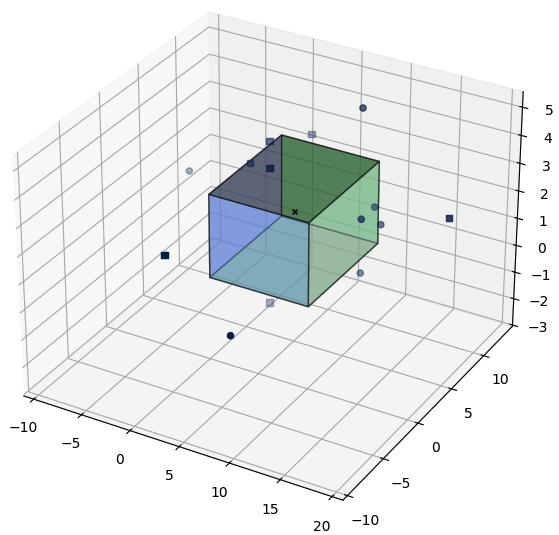
\includegraphics[width=0.75\linewidth]{diagrams/room.png}
    \caption{Room layout used in PyRoomAcoustics simulation.}
    \label{fig:doa_room_layout}
\end{figure}

\subsubsection{Test Data Generation}

After simulation, the multi-channel signals are saved as MP3 files
(\texttt{mic\_1.mp3}, \texttt{mic\_2.mp3}, \texttt{mic\_3.mp3},
\texttt{mic\_4.mp3}) in a directory named for the test case (e.g.,
\texttt{example\_mp3\_audio\_sources}). The \texttt{save\_room\_data()} function
in \texttt{pyroom\_helper.py} normalizes each channel to 16-bit integer range,
wraps it in a \texttt{pydub} \texttt{AudioSegment}, and exports to MP3. A
\texttt{README.md} is written alongside the audio files, documenting room
dimensions, microphone positions, source positions, and sampling frequency.
This metadata provides ground-truth DoA for validation.

The workflow is orchestrated by \texttt{example2.py}: create room, add
microphones, load or generate source signal, add source, simulate, optionally
plot the room and microphone responses, and save the data. The resulting files
are ``accurate'' in the sense that they are produced by a physics-based
simulation with known source and microphone geometry; the true azimuth can be
computed as $\theta_{\mathrm{true}} = \arctan2(x_s - x_c, y_s - y_c)$ where
$(x_s, y_s)$ is the source position and $(x_c, y_c)$ is the array center.

\begin{figure}[H]
    \centering
    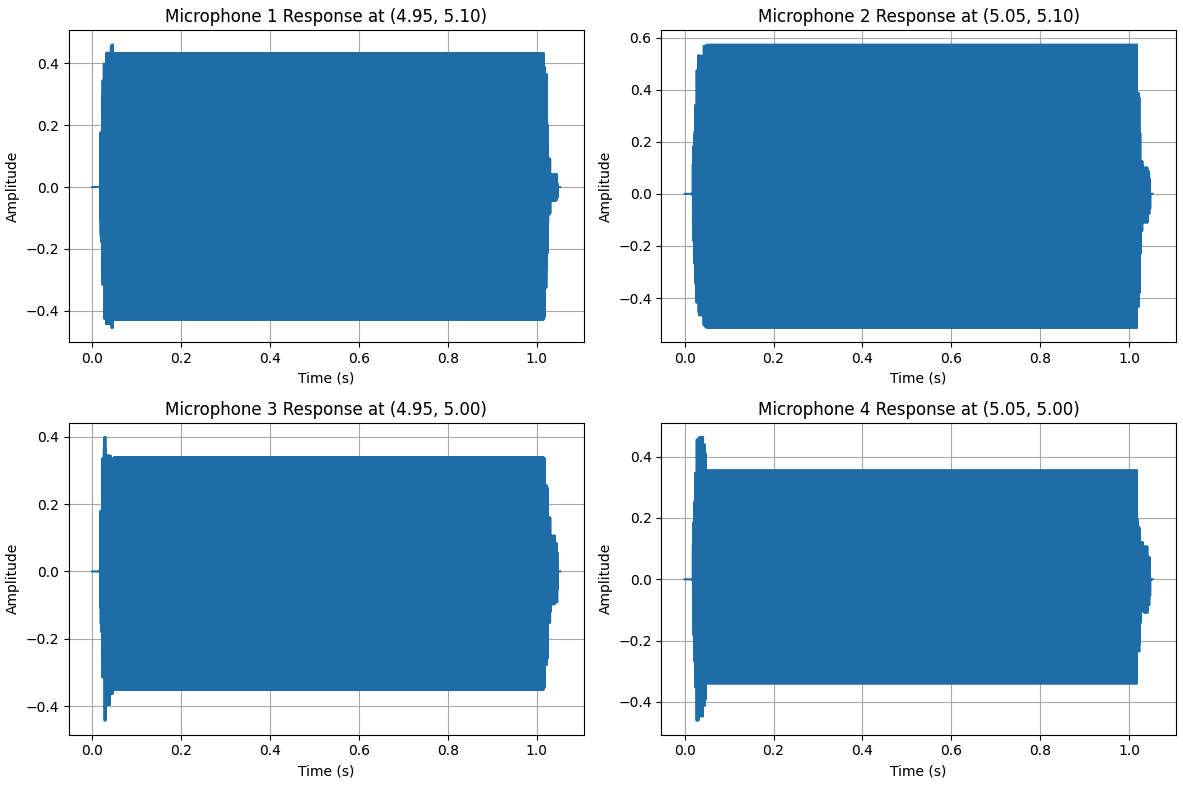
\includegraphics[width=0.9\linewidth]{diagrams/wave.png}
    \caption{Microphone responses after room simulation.}
    \label{fig:doa_mic_responses}
\end{figure}

\begin{figure}[H]
    \centering
    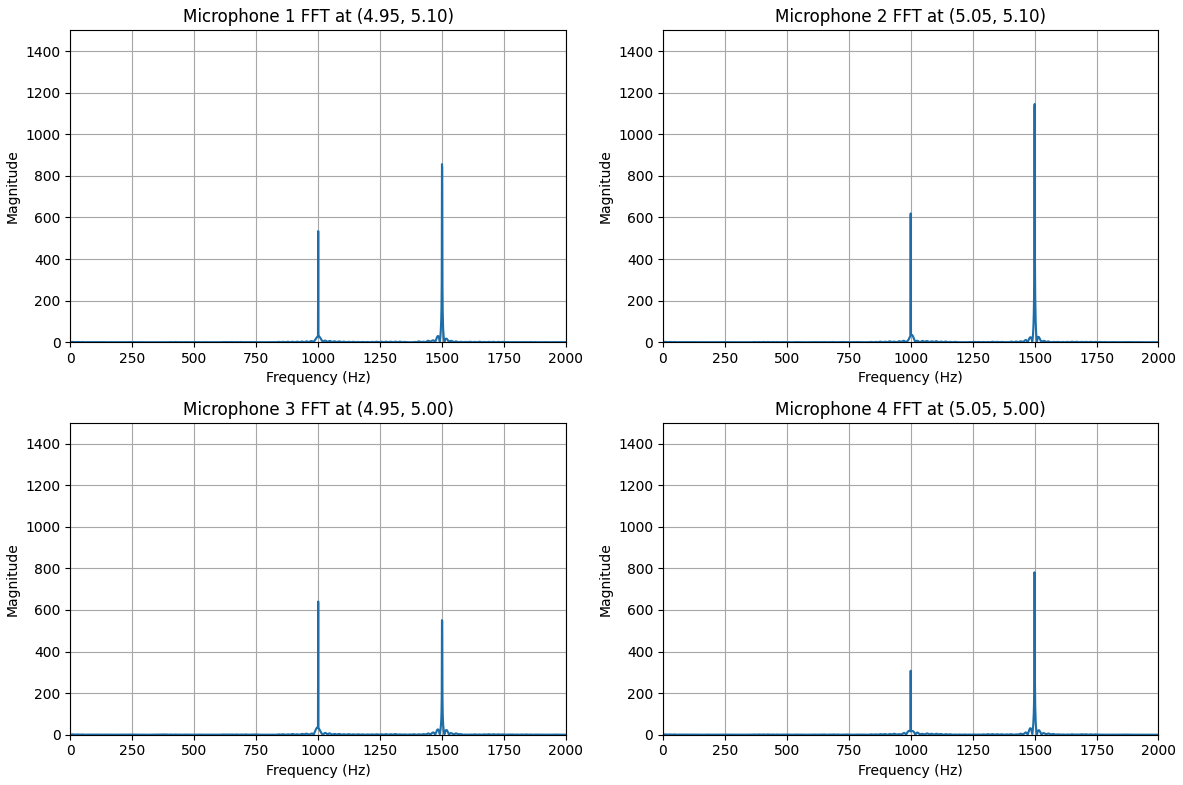
\includegraphics[width=0.9\linewidth]{diagrams/frequencies.png}
    \caption{Frequency-domain responses of microphone signals.}
    \label{fig:doa_mic_fft}
\end{figure}

\subsubsection{Algorithm Testing and Comparison}

The \texttt{doa\_analysis.py} module loads the saved MP3 files, normalizes
them to $[-1, 1]$, and converts the time-domain signals to the Short-Time
Fourier Transform (STFT) format required by pyroomacoustics DoA algorithms. The
STFT uses a Hanning window, FFT size $N_{\mathrm{FFT}} = 256$, and hop size
$N_{\mathrm{FFT}}/2$. The frequency range is restricted to $[300, 3000]$~Hz to
avoid DC and Nyquist aliasing and to focus on the most informative band for
speech and environmental sounds.

Each algorithm is invoked with the same STFT data and microphone array
geometry: \texttt{pra.doa.MUSIC}, \texttt{pra.doa.SRP}, and
\texttt{pra.doa.FRIDA}. The estimated azimuth angles are stored in
\texttt{doa\_obj.azimuth\_recon} (in radians). When a true source position is
provided, the true azimuth is computed and compared to the estimates.

The \texttt{example\_doa.py} script demonstrates the full pipeline: load data
from \texttt{example\_mp3\_audio\_sources}, run MUSIC, SRP-PHAT, and FRIDA, and
print a summary. The \texttt{visualize\_doa\_2d()} function produces a 2D polar
plot showing microphone positions, estimated directions (colored arrows), and
the true direction (black dashed arrow) when available.

\begin{figure}[H]
    \centering
    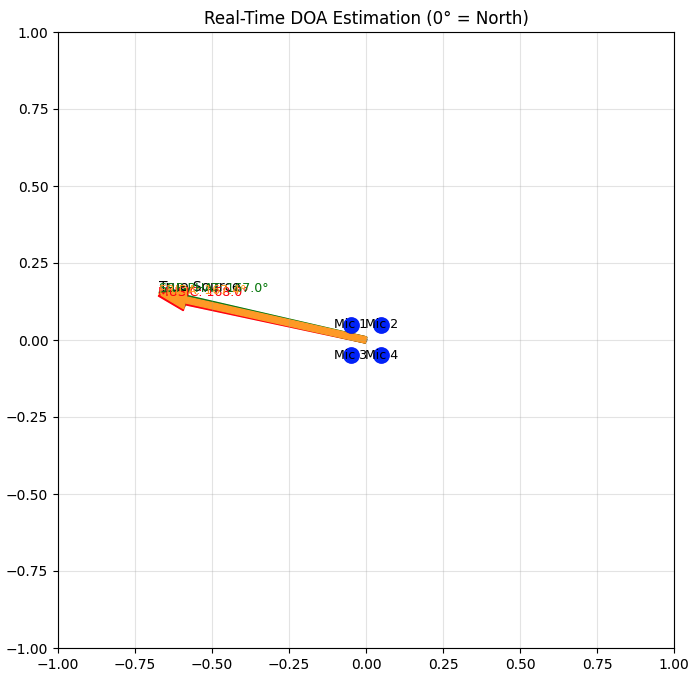
\includegraphics[width=0.75\linewidth]{diagrams/DOA.png}
    \caption{DoA estimation results: comparison of MUSIC, SRP-PHAT, and FRIDA
    with ground truth.}
    \label{fig:doa_visualization}
\end{figure}

The continuous simulation (\texttt{run\_simulation.py}) extends this workflow to
live audio: a microphone captures real-time input, which is convolved with
precomputed RIRs and fed to the DoA algorithms. The visualization updates
continuously as new direction estimates are produced. This mode supports
iterative tuning of algorithm parameters and validation under realistic
conditions.

\section{Classification}

\wss{This section is written by the classification partner.}

\newpage 
\bibliographystyle{IEEEtran}
\bibliography{../../../refs/References}

\end{document}